\documentclass[letterpaper,10pt]{article}

\usepackage{enumitem}
\usepackage{titling}
\usepackage{listings,listings-rust}
\usepackage{url}
\usepackage{soul}
\usepackage{hyperref}
\usepackage{setspace}
\usepackage{subfig}
\usepackage{sectsty}
\usepackage{pdfpages}
\usepackage{colortbl}
\usepackage{multirow}
\usepackage{multicol}
\usepackage{relsize}
\usepackage{amsmath}
\usepackage{wasysym}
\usepackage{fancyvrb}
\usepackage[yyyymmdd]{datetime}
\usepackage{amsmath,amssymb,amsthm,graphicx,xspace}
\usepackage[titlenotnumbered,noend,noline]{algorithm2e}
\usepackage[compact]{titlesec}
\usepackage{XCharter}
\usepackage[T1]{fontenc}
\usepackage[scaled]{beramono}
\usepackage[normalem]{ulem}
\usepackage{booktabs}
\usepackage{tikz}
\usetikzlibrary{arrows.meta,automata,shapes,trees,matrix,chains,scopes,positioning,calc,decorations.pathreplacing}
\tikzstyle{block} = [rectangle, draw, fill=blue!20, 
    text width=2.5em, text centered, rounded corners, minimum height=2em]
\tikzstyle{bw} = [rectangle, draw, fill=blue!20, 
    text width=4em, text centered, rounded corners, minimum height=2em]

\definecolor{namerow}{cmyk}{.40,.40,.40,.40}
\definecolor{namecol}{cmyk}{.40,.40,.40,.40}
\renewcommand{\dateseparator}{-}

\let\LaTeXtitle\title
\renewcommand{\title}[1]{\LaTeXtitle{\textsf{#1}}}

\lstset{basicstyle=\footnotesize\ttfamily,breaklines=true}

\newcommand{\CPP}{C\nolinebreak\hspace{-.05em}\raisebox{.4ex}{\tiny\bf +}\nolinebreak\hspace{-.10em}\raisebox{.4ex}{\tiny\bf +}}
\def\CPP{{C\nolinebreak[4]\hspace{-.05em}\raisebox{.4ex}{\tiny\bf ++}}}

\newcommand{\handout}[5]{
  \noindent
  \begin{center}
  \framebox{
    \vbox{
      \hbox to 5.78in { {\bf ECE459: Programming for Performance } \hfill #2 }
      \vspace{4mm}
      \hbox to 5.78in { {\Large \hfill #4  \hfill} }
      \vspace{2mm}
      \hbox to 5.78in { {\em #3 \hfill \today} }
    }
  }
  \end{center}
  \vspace*{4mm}
}

\newcommand{\lecture}[3]{\handout{#1}{#2}{#3}{Lecture#1}}
\newcommand{\tuple}[1]{\ensuremath{\left\langle #1 \right\rangle}\xspace}

\addtolength{\oddsidemargin}{-1.000in}
\addtolength{\evensidemargin}{-0.500in}
\addtolength{\textwidth}{2.0in}
\addtolength{\topmargin}{-1.000in}
\addtolength{\textheight}{1.75in}
\addtolength{\parskip}{\baselineskip}
\setlength{\parindent}{0in}
\renewcommand{\baselinestretch}{1.5}
\newcommand{\term}{Winter 2020}

\singlespace


\begin{document}

\lecture{19 --- Performance Case Studies}{\term}{Patrick Lam}

\section*{Making Firefox Fast}

Let's look at Mike Conley's Firefox Performance Updates,
\begin{center}
{\scriptsize
\vspace*{-1em}
\url{https://mikeconley.ca/blog/2018/02/14/firefox-performance-update-1/}
}
\end{center}
\vspace*{-1em}

\begin{itemize}[noitemsep]
\item don't use CPU animating out-of-view elements
\item move db init off main thread
\item keep better profiling data
\item parallel painting for macOS
\item lazily instantiate Search Service only when first search starts
\item halve size of the blocklist
\item refactor to reduce main-thread IO
\item don't hold all frames of animated GIFs/APNGs in memory
\item eliminate an unnecessary hash table
\item use more modern compiler
\end{itemize}

We can categorize most of these updates into the categories we've seen before:
\begin{itemize}[noitemsep]
\item do less work\\
 (or do it sooner/later);
\item use threads (move work off main thread);
\item track performance;
\end{itemize}
Which of the updates fall into which categories?

\subsection*{Tab warming} We continue by examining one particular update, \emph{tab warming}, in detail:
\begin{center}
\scriptsize
\vspace*{-1em}
\url{https://mikeconley.ca/blog/2018/01/11/making-tab-switching-faster-in-firefox-with-tab-warming/}.
\end{center}
\vspace*{-1em}

\hfill ``Maybe this is my Canadian-ness showing, but I like to think of it almost like coming in from shoveling snow off of the driveway, and somebody inside has \emph{already made hot chocolate for you}, because they knew you’d probably be cold.'' --- Mike Conley

Consider switching tabs. Previously, Firefox would request a paint of the newly-selected tab and wait for the rendering to be available before switching the tab.

The idea is to reduce user-visible latency by predicting an imminent tab switch. How do you know that the user is about to switch tabs? When the user has a mouse, then the mouse cursor will hover over the next tab.

\begin{quote}
Assuming a sufficiently long delay between hover and click, the tab switch should be perceived as instantaneous. If the delay was non-zero but still not long enough, we will have nonetheless shaved that time off in eventually presenting the tab to you.

And in the event that we were wrong, and you weren’t interested in seeing the tab, we eventually throw the uploaded layers away.
\end{quote}

The blog post does not report performance numbers (but bug 1430160 discusses how to collect them).

\subsection*{Firefox in general}

Try: ``about:mozilla'' in Firefox. On a Quantum Flow-enabled version, you'll see

\begin{center}
\emph{The Beast adopted new raiment and studied the ways of Time and Space and Light and the Flow of energy through the Universe. From its studies, the Beast fashioned new structures from oxidised metal and proclaimed their glories. And the Beast’s followers rejoiced, finding renewed purpose in these teachings.}

\hfill \emph{from The Book of Mozilla, 11:14}
\end{center}

In 2017, Mozilla released Electrolysis
(E10s\footnote{\url{https://blog.mozilla.org/blog/2017/06/13/faster-better-firefox/}}),
which leverages multicore processors by using multiple OS-level
processes. (Chrome has always done this, but Firefox attempts to also
keep memory usage
down\footnote{\url{https://medium.com/mozilla-tech/the-search-for-the-goldilocks-browser-and-why-firefox-may-be-just-right-for-you-1f520506aa35}}.)
Beyond internal architecture issues, handling Add-Ons (now
WebExtensions) was perhaps the most challenging part of going
multi-process.

Note the connection to different thread/process models.
Chrome is one-process-per-tab, while Firefox multiplexes tabs across
the 4 content processes (``hardware threads'', by analogy). Limiting
the number of tabs also limits the memory consumption of the browser:
we don't have arbitrary numbers of renderer state.

\begin{center}
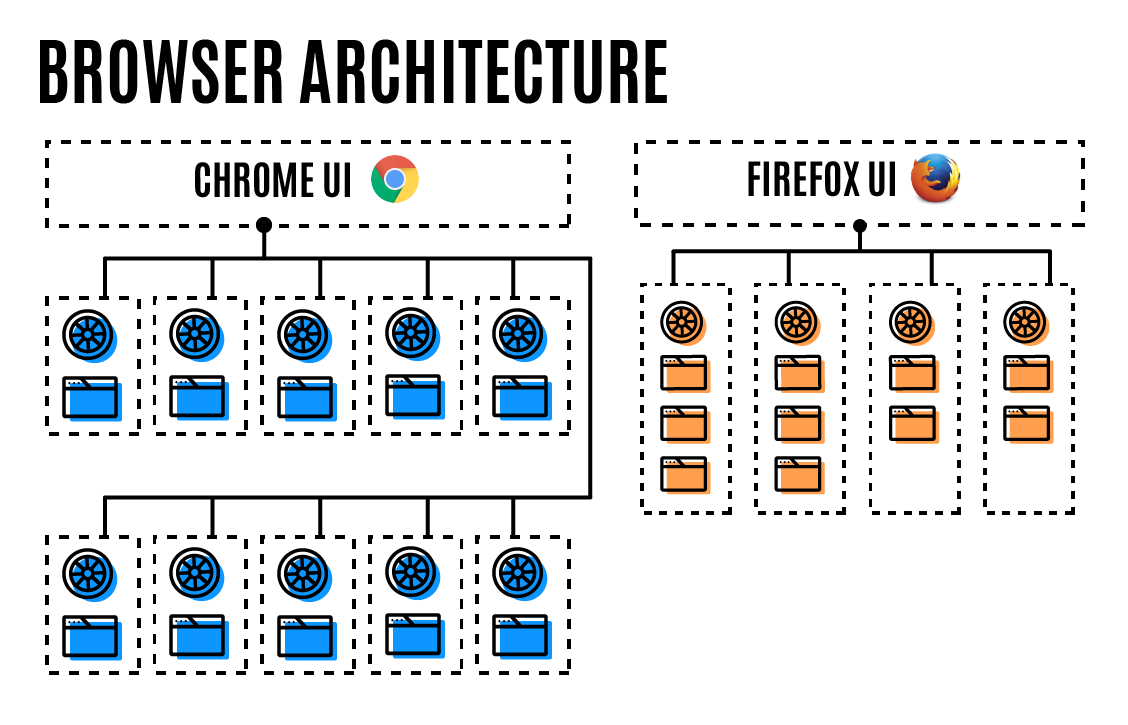
\includegraphics[width=.9\textwidth]{images/L19-chrome-vs-firefox.png}
\end{center}
Source: Ryan Pollock, ``The search for the Goldilocks browser and why Firefox might be `just right' for you'', \\
{\scriptsize \url{https://medium.com/mozilla-tech/the-search-for-the-goldilocks-browser-and-why-firefox-may-be-just-right-for-you-1f520506aa35}}

As a crude summary, Electrolysis works on splitting across processes
while the newer Quantum Flow leverages multithreading and other
improvements.  Quantum Flow uses the Rust programming language and its
``fearless concurrency'' (in Rust-speak). Rust should probably be part
of a future revision of the ECE 459 curriculum. But we'll focus on
Firefox here.

\subsection*{Quantum Flow}
Here's a retrospective of the Quantum Flow project:
\begin{center}
\url{https://ehsanakhgari.org/blog/2017-09-21/quantum-flow-engineering-newsletter-25}
\end{center}

To sum up, they formed a small term and did the following.
\begin{enumerate}[noitemsep]
\item Measure slowness: gather information, instrument Firefox, collect profiling data and measurements. Prioritize issues.
\item Gather help: convince other teams to pitch in with perf improvements. Examples: front-end team (reduce flushes, timers); layout team (reflow performance).
\item Fix all the things! (Or at least the most important ones).
\end{enumerate}
Given the short timeline they gave themselves (6 months) and the limited resources, an important part of their work was convincing others to help.
They triaged 895 bugs and fixed 369 of them. The weekly Quantum Flow Engineering Newsletter was a key motivational tool.

After the project wound down, they aimed to distribute responsibility for perf improvements across the entire project.

\section*{Firefox Telemetry}
Firefox's Telemetry feature collects lots of information from Firefox
users.  Idea: collect data before hacking away at things.  Firefox collects hundreds of
gigabytes of anonymous metrics per day while browsing and makes it all available to
the public.  One can view this as an analogy of CPU profiling on a
massively distributed context. This data is collected much less often than
CPU profiling data but at a much broader scope.
\begin{center}
\url{https://telemetry.mozilla.org/}
\end{center}
If you are running Firefox and want to see what it is collecting:
\begin{center}
\url{about:telemetry}
\end{center}

You can view distributions of telemetry probes (in the form of
histograms). You can also make your own dashboard based on Firefox
Telemetry data and Mozilla has infrastructure for their developres to
formulate and evaluate their own queries.

Example questions:
\begin{itemize}[noitemsep]
\item Is Firefox the user's default browser? (69\% yes)
\item Does e10s make startup faster? (no, slower)
\item Which plugins tend to freeze the browser on load? (Silverlight and Flash)
\end{itemize}
Can see evolution of data over time.

Firefox developers can propose new telemetry probes which are reviewed
for data privacy\footnote{Mozilla Data Collection Practices: \url{https://wiki.mozilla.org/Firefox/Data_Collection}} as well as through normal code review channels.

\paragraph{Pings.} Firefox phones the data home using so-called ``pings''.
Firefox sends a ``main ping'' every 24 hours, upon shutdown, environment change,
and crash. There are other types of pings as well. Pings get sent either by Firefox
or by a helper program, Pingsender, when Firefox isn't running. Presumably they
are sent over the network as compressed JSON to a central server.

Here's the common ping structure:

\begin{verbatim}
{
  type: <string>, // "main", "activation", "optout", "saved-session", ...
  id: <UUID>, // a UUID that identifies this ping
  creationDate: <ISO date>, // the date the ping was generated
  version: <number>, // the version of the ping format, currently 4

  application: {
    architecture: <string>, // build architecture, e.g. x86
    buildId: <string>, // "20141126041045"
    name: <string>, // "Firefox"
    version: <string>, // "35.0"
    displayVersion: <string>, // "35.0b3"
    vendor: <string>, // "Mozilla"
    platformVersion: <string>, // "35.0"
    xpcomAbi: <string>, // e.g. "x86-msvc"
    channel: <string>, // "beta"
  },

  clientId: <UUID>, // optional
  environment: { ... }, // optional, not all pings contain the environment
  payload: { ... }, // the actual payload data for this ping type
}
\end{verbatim}

Pings contain scalars (counts, booleans, strings) and histograms. A histogram collects
bucketed data (think grade distributions). Both scalars and histograms can be keyed, e.g.
how often searches happen for which search engines.



\section*{Single-Thread Performance}

\hfill ``Can you run faster just by trying harder?''

The performance improvements we've seen to date have been leveraging parallelism
to improve throughput. Decreasing latency is trickier---it often requires domain-specific
tweaks. Tab warming decreses latency but doesn't increase overall throughput.

Sometimes it's classic computer science: Quantum Flow found a place
where they could cache the last element of a list to reduce time
complexity for insertion from $O(n^2)$ to $O(n \log n)$.

\begin{center}
\url{https://bugzilla.mozilla.org/show_bug.cgi?id=1350770}
\end{center}

We'll also look at a more involved example of decreasing latency today, Stream VByte~\cite{LEMIRE20181}.
Even this example leverages parallelism---it uses vector instructions. But there
are some sequential improvements, e.g. Stream VByte takes care to be predictable
for the branch predictor.

\paragraph{Context.} We can abstract the problem to that of storing a sequence of small integers.
Such sequences are important, for instance, in the context of inverted indexes, which allow
fast lookups by term, and support boolean queries which combine terms.

Here is a list of documents and some terms that they contain:
\begin{center}
\begin{tabular}{r|l}
docid & terms \\ \hline
1 & dog, cat, cow\\
2 & cat\\
3 & dog, goat\\
4 & cow, cat, goat\\
\end{tabular}
\end{center}

The inverted index looks like this:
\begin{center}
\begin{tabular}{r|l}
term & docs \\ \hline
dog & 1, 3 \\
cat & 1, 2, 4 \\
cow & 1, 4 \\
goat & 3, 4
\end{tabular}
\end{center}

Inverted indexes contain many small integers in their lists: it is
sufficient to store the delta between a doc id and its successor, and
the deltas are typically small if the list of doc ids is sorted.
(Going from deltas to original integers takes time logarithmic
in the number of integers).

VByte is one of a number of schemes that use a variable number of
bytes to store integers.  This makes sense when most integers are
small, and especially on today's 64-bit processors.

VByte works like this:
\vspace*{-1em}
\begin{itemize}[noitemsep]
\item $x$ between 0 and $2^7-1$, e.g. $17 = 0b10001$: $0xxx xxxx$, e.g. $0001 0001$;
\item $x$ between $2^7$ and $2^{14}-1$, e.g. $1729 = 0b110 11000001$:
                   $1xxx xxxx/0xxx xxxx$, e.g. $1100 0001/0000 1101$;
\item $x$ between $2^{14}$ and $2^{21}-1$: $0xxx xxxx/1xxx xxxx/1xxx xxxx$;
\item etc.
\end{itemize}
That is, the control bit, or high-order bit, is 0 if you have finished representing the integer,
and 1 if more bits remain. (UTF-8 encodes the length, from 1 to 4, in high-order bits of the first byte.)

It might seem that dealing with variable-byte integers might be
harder than dealing fixed-byte integers, and it is. But there are performance benefits: because we are
using fewer bits, we can fit more information into our limited RAM and
cache, and even get higher throughput. Storing and reading 0s isn't an effective
use of resources. However, a naive algorithm to decode VByte also gives
lots of branch mispredictions.

Stream VByte is a variant of VByte which works using SIMD instructions.
Science is incremental, and Stream VByte builds on earlier work---masked VByte
as well as {\sc varint}-GB and {\sc varint}-G8IU. The innovation in
Stream VByte is to store the control and data streams separately.

Stream VByte's control stream uses two bits per integer to represent the size of the integer:
\begin{center}
\vspace*{-1em}
\begin{tabular}{ll@{~~~~~~~~}ll}
00 & 1 byte & 10 & 3 bytes\\
01 & 2 bytes & 11 & 4 bytes
\end{tabular}
\end{center}

Each decode iteration reads a byte from the control stream and 16 bytes of data from memory.
It uses a lookup table over the possible values of the control stream to decide how many
bytes it needs out of the 16 bytes it has read, and then uses SIMD instructions to shuffle
the bits each into their own integers. Note that, unlike VByte, Stream VByte uses all 8 bits
of each data byte as data.

For instance, if the control stream contains $0b1000~1100$, then the data stream
contains the following sequence of integer sizes: $3, 1, 4, 1$. Out of the 16 bytes read,
this iteration will use 9 bytes; it advances the data pointer by 9. It then uses the SIMD
``shuffle'' instruction to put the decoded integers from the data stream at known positions in the
128-bit SIMD register; in this case, it pads the first 3-byte integer with 1 byte, then
the next 1-byte integer with 3 bytes, etc. Let's say that the input is
{\tt 0xf823~e127~2524~9748~1b..~....~....~....}. The 128-bit output is
{\tt 0x00f8~23e1/0000~0027/2524 9748/0000/001b}, with the /s denoting separation
between outputs. The shuffle mask is precomputed and, at
execution time, read from an array.

The core of the implementation uses three SIMD instructions:
\begin{lstlisting}[language=C]
  uint8_t C = lengthTable[control];
  __m128i Data = _mm_loadu_si128 ((__m128i *) databytes);
  __m128i Shuf = _mm_loadu_si128(shuffleTable[control]);
  Data = _mm_shuffle_epi8(Data, Shuf);
  databytes += C; control++;
\end{lstlisting}

\paragraph{Discussion.} The paper~\cite{LEMIRE20181} includes a number of benchmark results
showing how Stream VByte performs better than previous techniques on a realistic input.
Let's discuss how it achieves this performance.

\begin{itemize}[noitemsep]
\item control bytes are sequential: the processor can always prefetch the next control byte, because
its location is predictable;
\item data bytes are sequential and loaded at high throughput;
\item shuffling exploits the instruction set so that it takes 1 cycle;
\item control-flow is regular (executing only the tight loop which retrieves/decodes control
and data; there are no conditional jumps).
\end{itemize}
We're exploiting SIMD, so this isn't quite strictly single-threaded performance.
Considering branch prediction and caching issues, though,
certainly improves single-threaded performance.


\bibliographystyle{alphaurl}
\bibliography{459}


\end{document}
